\documentclass[aspectratio=169]{beamer}
\usepackage[utf8]{inputenc}
\usetheme{Madrid}
\usepackage{xcolor}
\usepackage{listings}
\usepackage{tikz}
\usetikzlibrary{positioning,shapes,arrows}

\definecolor{IBMBlue}{RGB}{0,113,197}
\setbeamercolor{structure}{fg=IBMBlue}

\author[J. Woźniak]{mgr inż. Jakub Woźniak}
\institute[PUT]{Politechnika Poznańska\\Wydział Informatyki i Telekomunikacji}
\date{}
\title{CI/CD i automatyzacja procesów deweloperskich}
\subtitle{definicja problemu i strategie}


\usepackage{booktabs} % Do ładnych tabel


\setbeamertemplate{navigation symbols}{} % Ukrycie paska nawigacji
\setbeamertemplate{headline}{} % Czysty nagłówek

% --- Konfiguracja listingu (YAML) ---
\definecolor{eclipseBlue}{RGB}{42,0.0,255}
\definecolor{eclipseGreen}{RGB}{63,127,95}
\definecolor{eclipsePurple}{RGB}{127,0,85}
\lstdefinelanguage{yaml}{
  keywords={true,false,null,y,n},
  keywordstyle=\color{darkgray}\bfseries,
  basicstyle=\ttfamily\footnotesize,                                 
  breaklines=true,
  breakatwhitespace=false,
  captionpos=b,
  commentstyle=\color{eclipseGreen},
  stringstyle=\color{eclipseBlue},
  identifierstyle=\color{black},
  showstringspaces=false,
  backgroundcolor=\color{gray!10},
  frame=single,
  rulecolor=\color{gray!30},
}


\begin{document}

% --- Slajd Tytułowy ---
\begin{frame}
    \titlepage
\end{frame}

% --- Agenda ---
\begin{frame}{Agenda Wykładu}
    \tableofcontents
\end{frame}

% ==============================================================================
\section{Wstęp: Kryzys Skali i Ewolucja}
% ==============================================================================

\begin{frame}{Ewolucja: Od Skryptów do Platform Engineeringu}
    \begin{columns}
        \column{0.5\textwidth}
        \textbf{Era DevOps (2015-2020):}
        \begin{itemize}
            \item "You build it, you run it".
            \item Każdy zespół pisze własne pipeline'y (Jenkinsfile).
            \item Problem: Kognitywne przeciążenie deweloperów.
        \end{itemize}
        
        \column{0.5\textwidth}
        \textbf{Era Platform Engineering (2025):}
        \begin{itemize}
            \item Traktowanie platformy jako produktu.
            \item \textbf{IDP (Internal Developer Platform):} Backstage, Port.
            \item \textit{Golden Paths}: Prekonfigurowane szablony usług.
        \end{itemize}
    \end{columns}
    
    \vspace{1em}
    \begin{alertblock}{Kluczowa zmiana}
        Przesuwamy ciężar z \textit{konfiguracji imperatywnej} na \textit{abstrakcję platformową}.
    \end{alertblock}
\end{frame}

\begin{frame}{Jak mierzyć sukces? Metryki DORA w systemach rozproszonych}
    \begin{table}[]
        \centering
        \resizebox{\textwidth}{!}{
        \begin{tabular}{@{}lll@{}}
            \toprule
            \textbf{Metryka} & \textbf{Definicja} & \textbf{Wyzwanie w skali mikroserwisów} \\ \midrule
            \textbf{Deployment Frequency} & Częstotliwość wdrożeń & Agregacja wdrożeń 100+ serwisów vs Monolit \\
            \textbf{Lead Time for Changes} & Czas od commitu do prod & Zależności "Train Release Model" \\
            \textbf{Change Failure Rate} & \% awaryjnych wdrożeń & Kaskada błędów między serwisami \\
            \textbf{Mean Time to Recovery} & Średni czas naprawy & Distributed Tracing (Root Cause Analysis) \\ \bottomrule
        \end{tabular}
        }
    \end{table}
\end{frame}

% ==============================================================================
\section{Inżynieria Budowania - Build Engineering}
% ==============================================================================

\begin{frame}{Architektura Repozytorium: Monorepo vs Polyrepo}
    \begin{columns}
        \column{0.5\textwidth}
        \textbf{Polyrepo (Wiele repozytoriów)}
        \begin{itemize}
            \item Izolacja usług.
            \item Niezależne cykle wydawnicze.
            \item \textcolor{red}{Wada: "Dependency Hell" przy aktualizacji bibliotek współdzielonych.}
        \end{itemize}
        
        \column{0.5\textwidth}
        \textbf{Monorepo (Jedno repozytorium)}
        \begin{itemize}
            \item Atomowe zmiany (API + Klient w jednym commicie).
            \item Ujednolicone wersjonowanie.
            \item \textcolor{red}{Wada: Czas budowania rośnie wykładniczo bez odpowiednich narzędzi.}
        \end{itemize}
    \end{columns}
\end{frame}

\begin{frame}{Inteligentne Budowanie: Dependency Graph Analysis}
    Nie budujemy wszystkiego (`build all`). Budujemy tylko to, co się zmieniło (`build affected`).
    
    \begin{center}
    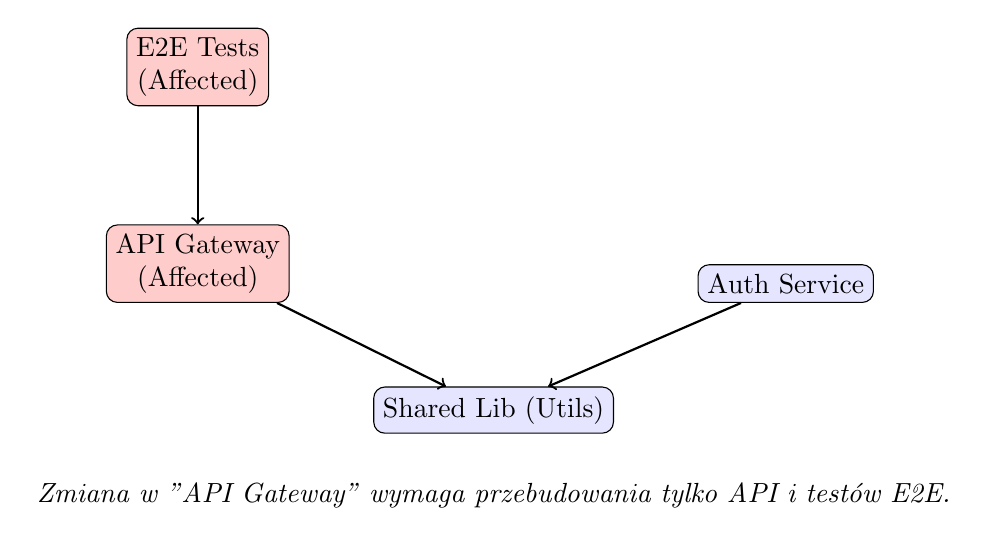
\begin{tikzpicture}[
        node distance=1.5cm,
        every node/.style={rectangle, draw, rounded corners, align=center},
        affected/.style={fill=red!20},
        normal/.style={fill=blue!10}
    ]
        \node[normal] (util) {Shared Lib (Utils)};
        \node[affected, above left=of util] (api) {API Gateway\\(Affected)};
        \node[normal, above right=of util] (auth) {Auth Service};
        \node[affected, above=of api] (e2e) {E2E Tests\\(Affected)};
        
        \draw[->, thick] (api) -- (util);
        \draw[->, thick] (auth) -- (util);
        \draw[->, thick] (e2e) -- (api);
        
        \node[below=0.5cm of util, draw=none, fill=none] {\textit{Zmiana w "API Gateway" wymaga przebudowania tylko API i testów E2E.}};
    \end{tikzpicture}
    \end{center}
    
    \textbf{Narzędzia:} Bazel, Nx, Gradle Enterprise, Turborepo.
\end{frame}

\begin{frame}{Hermetic Builds & Remote Caching}
    \textbf{Hermetyczność:} Proces budowania zależy \textit{wyłącznie} od zadeklarowanych wejść (kod, narzędzia). Brak dostępu do sieci i `/usr/bin`.
    
    \vspace{1em}
    \textbf{Remote Caching (Zdalne buforowanie):}
    \begin{enumerate}
        \item Oblicz Hash = $H(Source Files + Env Vars + Compiler Flags)$.
        \item Sprawdź w Cache (S3/Redis).
        \item \textbf{Hit:} Pobierz artefakt (sekundy).
        \item \textbf{Miss:} Buduj i wyślij do cache (minuty).
    \end{enumerate}
    
    \begin{block}{Efekt skali}
        Jeśli kolega z zespołu już zbudował bibliotekę `common-math`, Twój build pobierze gotowy plik binarny.
    \end{block}
\end{frame}

% ==============================================================================
\section{GitOps i Model Rekoncyliacji}
% ==============================================================================

\begin{frame}{Paradygmat GitOps: Push vs Pull}
    \begin{columns}
        \column{0.5\textwidth}
        \textbf{CIOps (Push Model - np. Jenkins)}
        \begin{itemize}
            \item CI ma `kubectl apply`.
            \item CI ma "klucze do królestwa".
            \item \textbf{Configuration Drift:} CI nie wie, jeśli ktoś zmienił coś ręcznie na klastrze.
        \end{itemize}
        
        \column{0.5\textwidth}
        \textbf{GitOps (Pull Model - np. ArgoCD)}
        \begin{itemize}
            \item Agent działa \textit{wewnątrz} klastra.
            \item Git jako jedyne źródło prawdy (SSOT).
            \item \textbf{Reconciliation Loop:} Ciągłe porównywanie stanu Git ze stanem klastra.
        \end{itemize}
    \end{columns}
\end{frame}

\begin{frame}[fragile]{Pętla Rekoncyliacji (The Reconciliation Loop)}
    GitOps to implementacja teorii sterowania w inżynierii oprogramowania.
    
    \begin{center}
    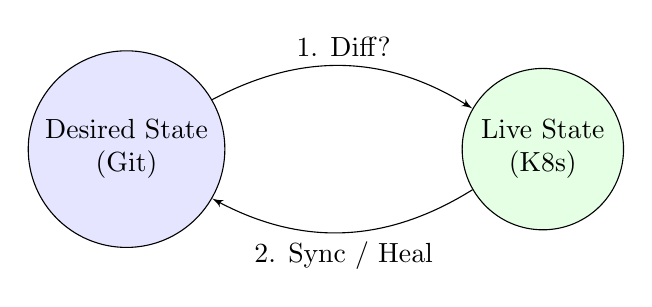
\begin{tikzpicture}[auto, node distance=2cm,>=latex']
        \node [draw, circle, fill=blue!10, align=center] (desired) {Desired State\\(Git)};
        \node [draw, circle, fill=green!10, align=center, right=3cm of desired] (live) {Live State\\(K8s)};
        
        \path[->] (desired) edge [bend left] node {1. Diff?} (live);
        \path[->] (live) edge [bend left] node {2. Sync / Heal} (desired);
    \end{tikzpicture}
    \end{center}
\end{frame}
\begin{frame}[fragile]{Pętla Rekoncyliacji (The Reconciliation Loop) - kont.}
    \textbf{Przykład obiektu ArgoCD Application:}
    \begin{lstlisting}[language=yaml]
apiVersion: argoproj.io/v1alpha1
kind: Application
spec:
  source:
    repoURL: https://github.com/my-org/infra.git
    path: k8s/overlays/prod
  destination:
    server: https://kubernetes.default.svc
  syncPolicy:
    automated:
      prune: true      # Usuń zasoby, których nie ma w Git
      selfHeal: true   # Napraw, jeśli ktoś zmienił ręcznie
    \end{lstlisting}
\end{frame}

\begin{frame}{Zarządzanie Sekretami w GitOps}
    Nie możemy trzymać haseł jawnym tekstem w Git. Dwa podejścia:
    
    \begin{enumerate}
        \item \textbf{Szyfrowanie w Git (Sealed Secrets):}
            \begin{itemize}
                \item Szyfrujemy kluczem publicznym klastra.
                \item Tylko kontroler w klastrze ma klucz prywatny.
                \item Plik w repozytorium jest bezpieczny.
            \end{itemize}
        \item \textbf{Zewnętrzny Skarbiec (External Secrets Operator):}
            \begin{itemize}
                \item Sekrety w AWS Secrets Manager / HashiCorp Vault.
                \item W Git tylko referencja (wskaźnik).
                \item Operator pobiera sekret i wstrzykuje go jako Kubernetes Secret.
            \end{itemize}
    \end{enumerate}
\end{frame}

% ==============================================================================
\section{Strategie Progresywnego Dostarczania}
% ==============================================================================

\begin{frame}{Deployment vs Release}
    \begin{alertblock}{Kluczowe rozróżnienie}
        \textbf{Deployment (Wdrożenie):} Instalacja nowej wersji oprogramowania na infrastrukturze (czynność techniczna).
        
        \textbf{Release (Wydanie):} Udostępnienie funkcjonalności użytkownikom (decyzja biznesowa).
    \end{alertblock}
    
    W systemach rozproszonych unikamy "Big Bang Deployments" (wszyscy naraz). Stosujemy \textbf{Progressive Delivery}.
\end{frame}

\begin{frame}{Strategie Wdrożeń}
    \begin{table}[]
        \centering
        \resizebox{\textwidth}{!}{
        \begin{tabular}{@{}llll@{}}
            \toprule
            \textbf{Strategia} & \textbf{Mechanizm} & \textbf{Zalety} & \textbf{Wady} \\ \midrule
            \textbf{Rolling Update} & Stopniowa wymiana Podów & Standard w K8s, brak downtime & Trudny rollback, brak testów na grupie \\
            \textbf{Blue/Green} & Dwa środowiska, przełącznik LB & Błyskawiczny rollback & Koszt (2x zasoby) \\
            \textbf{Canary} & Przekierowanie \% ruchu & Minimalny "Blast Radius" & Złożona konfiguracja (Service Mesh) \\ \bottomrule
        \end{tabular}
        }
    \end{table}
\end{frame}

\begin{frame}[fragile]{Argo Rollouts: Canary Analysis}
    Rozszerzenie standardowego `Deployment` w Kubernetes. Pozwala na automatyczną analizę metryk.
    
    \begin{lstlisting}[language=yaml]
apiVersion: argoproj.io/v1alpha1
kind: Rollout
spec:
  strategy:
    canary:
      steps:
      - setWeight: 20
      - pause: {duration: 5m}
      - analysis:
          templates:
          - templateName: success-rate # Sprawdź Prometheus
      - setWeight: 50
      - pause: {duration: 10m}
    \end{lstlisting}
    
    Jeśli `success-rate` spadnie poniżej 99\%, nastąpi \textbf{automatyczny rollback}.
\end{frame}

% ==============================================================================
\section{Zarządzanie Stanem i Bazy Danych}
% ==============================================================================

\begin{frame}{Problem Stanu w CI/CD}
    Aplikację (Stateless) łatwo cofnąć (`git revert`).
    Bazy danych (Stateful) nie da się cofnąć bez utraty danych transakcyjnych.
    
    \vspace{1em}
    \textbf{Wzorzec Expand-Contract (Parallel Change):}
    \begin{enumerate}
        \item \textbf{Expand:} Dodaj nową kolumnę/tabelę. Stara nadal istnieje. (Baza obsługuje v1 i v2).
        \item \textbf{Deploy:} Wdróż aplikację v2 (pisze do nowej, czyta z nowej, fallback do starej).
        \item \textbf{Migrate:} Przepisz stare dane (Backfill).
        \item \textbf{Contract:} Usuń starą kolumnę w kolejnym sprincie.
    \end{enumerate}
    
    \textit{Zasada:} Baza danych musi być zawsze kompatybilna wstecz o N-1 wersji.
\end{frame}

\begin{frame}{Kubernetes StatefulSets}
    Dla baz danych (Postgres, Cassandra, Kafka) na K8s używamy `StatefulSet`.
    
    \textbf{Różnice w aktualizacji:}
    \begin{itemize}
        \item Pods mają stałą tożsamość (`kafka-0`, `kafka-1`).
        \item Aktualizacja jest sekwencyjna (od końca: 2 -> 1 -> 0).
        \item CI/CD musi czekać na `Ready` check każdego węzła, aby zachować kworum klastra (np. Raft consensus).
    \end{itemize}
\end{frame}

% ==============================================================================
\section{Podsumowanie}
% ==============================================================================

\begin{frame}{Podsumowanie Wykładu}
    \begin{enumerate}
        \item \textbf{Kryzys skali:} Tradycyjne CI (Jenkins) nie skaluje się dla 100+ mikroserwisów. Platform Engineering i IDP to odpowiedź.
        \item \textbf{Build Engineering:} Wymaga podejścia grafowego (Bazel/Nx) i zdalnego cache'owania.
        \item \textbf{GitOps:} To standard operacyjny. Klaster sam naprawia swój stan (Reconciliation Loop).
        \item \textbf{Progressive Delivery:} Odseparowanie wdrożenia od wydania. Automatyczna analiza Canary zmniejsza ryzyko awarii.
        \item \textbf{Bazy danych:} Są najtrudniejszym elementem. Wymagają migracji Zero-Downtime (Expand-Contract).
    \end{enumerate}
\end{frame}

\begin{frame}{Pytania i dyskusja}
    \begin{center}
        \Huge Dziękuję za uwagę.
    \end{center}
\end{frame}

\end{document}
